%
% 05_reell_analytische_kurven.tex -- Einfuhrung in den Satz von Jordan fuer reell-analytische Kurven
%
% (c) 2026 Dominik Castelberg, Ostschweizer Fachhochschule
%
% !TEX root = ../../buch.tex
% !TEX encoding = UTF-8
%

\section{Der Fall reell-analytischer Kurven
\label{jordan:section:reell_analytische_kurven}}
\kopfrechts{Der Fall reell-analytischer Kurven}

Mit dem Schritt von einfachen Polygonen zu reell-analytischen Kurven (im Folgenden als $\gamma$ bezeichnet) verlieren wir mehrere Eigenschaften und Werkzeuge, welche wir bisher für die Beweisführung verwendet haben. 

Spezifisch verlieren wir:

\begin{itemize}
    \item \textbf{Strahlenparität:} Die Zahl der Schnittpunkte eines Strahls mit $\gamma$ ist nicht mehr offensichtlich endlich, da $\gamma$ keine Kanten mehr hat. 
    \item \textbf{Triangulierung:} Es gibt keine kanonische Triangulierung von $I$ mit Ecken auf $\gamma$, weil $\gamma$ keine Ecken hat. 
    \item \textbf{Diagonal-Lemma:} Aus dem gleichen Grund ist das Konzept einer Diagonale nicht mehr anwendbar.
\end{itemize}

Entsprechend stehen wir vor einer Wegzweigung: Entweder wir erweitern das Werkzeug der Strahlenparität, sodass es auf reell-analytische Kurven anwendbar ist, oder wir finden ein neues Werkzeug, das die Strahlenparität ersetzt. 
Wir werden in diesem Abschnitt beide Ansätze diskutieren dabei herausfinden, dass einer der Ansätze dabei deutlich eleganter ist. 

Zusätzlich erhalten wir dank der Reell-Analytizität von $\gamma$ eine neue Kiste von analytischen Werkzeugen, die wir für unsere Beweisführung verwenden können:

\subsection{Fortführung des Strahlenparität-Arguments}

Um die Strahlenparität weiter zu entwickeln, betrachten wir die Wirkung von Deformationen auf die Anzahl der Schnittpunkte zwischen einer Kurve und einem Strahl. 
Hierfür verwenden wir zwei neue, analytische Werkzeuge: Die endliche Schnittstruktur und die Tubulare Umgebung. 

\begin{satz}[Endliche Schnittstruktur\label{jordan:satz:endliche_schnittstruktur}]
\index{endliche Schnittstruktur}%
\index{Satz!endliche Schnittstruktur}%
    Sei $\gamma$ eine reell-analytische Kurve in der Ebene $\mathbb{R}^2$ und $L$ ein Strahl mit Anfangspunkt $p \in \mathbb{R}^2$.
    Dann ist $\gamma \cap L$ endlich. Ausnahmefall ist $\gamma \cap L = \emptyset$.
\end{satz}


\begin{satz}[Identitätssatz für reell-analytische Funktionen\label{jordan:satz:identitaetssatz_reell_analytische_funktionen}]
    Sei $f: U \subset \mathbb{R} \to \mathbb{R}$ eine nicht verschwindende reell-analytische Funktion auf einer zusammenhängenden Menge $U$.
    Die Nullstellen von $f$ auf $U$ sind diskret und auf einer kompakten Teilmenge von $U$ somit endlich.
\end{satz}

Da $\gamma \cap L = \emptyset$ bei geschlossenen Kurven nicht auftreten kann, und der Satz von Jordan eine geschlossene Kurve $\gamma$ voraussetzt, gilt der Satz der endlichen Schnittstruktur für sämtliche für uns relevanten Kurven. 

Mit der endlichen Schnittstruktur können wir garantieren, dass die Anzahl der Schnittpunkte zwischen einem Strahl und einer reell-analytischen Kurve endlich ist. 
Dies ist ein wichtiger Schritt in der Fortführung des Strahlenparitäts-Arguments, da mit der Modulo-Rechnung unser Mittel, die Parität der Schnittpunkte zu analysieren, nur auf endliche Mengen anwendbar ist. 

Mit dem Beweis der endlichen Schnittstruktur abgeschlossen, können wir nun die Tubulare Umgebung einführen, die es uns erlaubt, die Strahlenparität auf reell-analytische Kurven zu erweitern.

\begin{lemma}[Existenz einer tubularen Umgebung\label{jordan:lemma:tubulare_umgebung}]
    Sei $\gamma$ eine reell-analytische Kurve in der Ebene $\mathbb{R}^2$. Dann existiert $\varepsilon > 0$, so dass die Abbildung $\varphi: S\textsuperscript{1} \times (-\varepsilon, \varepsilon) \to \mathbb{R}^2$, $\varphi(t,s) = \gamma(t) + s \cdot n(t)$, ein reell-analytischer Diffeomorphismus auf eine offene Umgebung $T$ von $\gamma$ ist, wobei $n(t)$ der nach aussen gerichtete Einheitsnormalenvektor ist. 
    Das Komplement $T \setminus \gamma$ zerfällt in zwei zusammenhängende Komponenten entsprechend $s > 0$ und $s < 0$, die als innere und äussere tubulare Umgebung bezeichnet werden.    
\end{lemma}

Das Komplement $T \setminus \gamma$ zerfällt in zwei zusammenhängende Komponenten entsprechend $s > 0$ und $s < 0$, die als innere und äussere tubulare Umgebung bezeichnet werden.

\begin{figure}
    \centering
    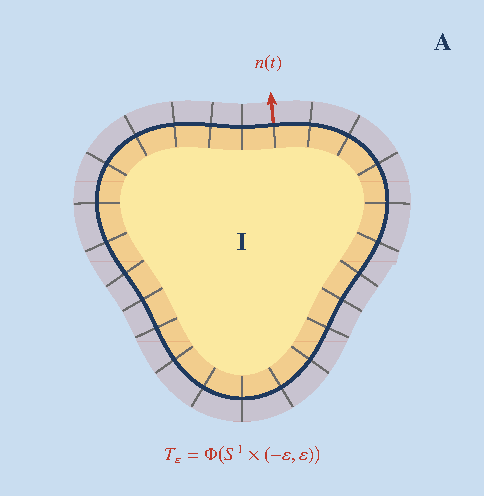
\includegraphics{papers/jordan/images/tubulare_umgebung.pdf}
    \caption{Die tubulare Umgebung einer reell-analytischen Kurve.}
\end{figure}

Das Lemma der tubularen Umgebung kann mithilfe der Determinanten der im Abschnitt \ref{buch:holomoprh:holomorph:subsection:komplexedifferenzierbarkeit} eingeführten Jacobi-Matrix bewiesen werden.  

Mit diesen Werkzeugen können wir die Strahlenparität auf reell-analytische Kurven erweitern.
Bewiesen wird dies über die endliche Schnittstruktur. Für $p \in \mathbb{R}^2 \setminus \gamma$ wählen wir einen Strahl $L$ mit Anfangspunkt $p$, der nicht tangential an $\gamma$ verläuft und durch keinen degenerierten Punkt von $\gamma$ geht.
Gemäss der endlichen Schnittstruktur ist die Anzahl der Schnittpunkte $N(p,L)$ immer diskret, also ist jede Richtung zulässig. 
Da die Schnittstruktur endlich ist, ist die Parität $N(p,L) \mod 2$ wieder wohldefiniert und hängt nicht von der Wahl des Strahls ab. 

Der Wegzusammenhang von $I$ und $A$, genauso wie die Beschränktheit von $I$, ergeben sich aus der Konstruktion der tubulären Umgebung. 
Die Beweise der Offenheit von $I$ und $A$, genauso wie die Unbeschränktheit von $A$, haben sich gegenüber \ref{jordan:section:einfache_polygone} nicht verändert.

Diese Beweisstrategie funktioniert, aber leider ist er auch analytisch aufwendig:

\begin{itemize}
    \item Fallunterscheidung zu Tangentenschnitten
    \item Kontrolle der Paritätsinvarianz unter Strahlendeformationen
    \item Genaue Analyse entarteter Strahlrichtungen
\end{itemize}

All diese Punkte verlangen sorgfältige analytische Arbeit, welche im polygonalen Fall durch die kombinatorische Endlichkeit ersetzt war. 
Entsprechend werden wir uns nun einem alternativen Ansatz, der uns mit seiner Eleganz viel Arbeit erspart, zuwenden. 

\subsection{Nutzung der Umlaufzahl statt der Strahlenparität}

Im Abschnitt \ref{buch:integration:cauchy:subsetion:umlaufzahl} wurde die Umlaufzahl eines Weges um einen Punkt eingeführt. 
Diese Umlaufzahl besitzt Eigenschaften, die es uns erlauben, die Strahlenparität als Argument komplett zu verwerfen. 

\begin{lemma}[Grundlegende Eigenschaften der Umlaufzahl\label{jordan:lemma:grundlegende_eigenschaften_umlaufzahl}]
    Für jede geschlossene, stückweise C\textsuperscript{1}-Kurve $\gamma$ mit Umlaufzahl $n(\gamma, z)$ und $z \notin \gamma$ gilt:
    \begin{enumerate}
        \item $n(\gamma, z) \in \mathbb{Z}$
        \item Die Abbildung $z \mapsto n(\gamma, z)$ ist lokal konstant auf $\mathbb{C} \setminus \gamma$.
        \item Für $|z|$ hinreichend gross gilt $n(\gamma, z) = 0$.
    \end{enumerate}

\end{lemma}

Aus diesen Eigenschaften folgt schon fast der Satz von Jordan im analytischen Fall: Die Funktion $z \mapsto n(\gamma, z)$ nimmt auf jeder zusammenhängenden Komponente von $\mathbb{C} \setminus \gamma$ einen konstanten ganzzahligen Wert an. 
Auf der unbeschränkten Komponente ist dieser Wert $0$. 

Für einen vollständigen Beweis müssen wir jedoch noch zeigen, dass es mindestens eine Komponente gibt, auf der $n(\gamma, z) \neq 0$ gilt und dass es auf jeder beschränkten Komponente den Wert $\pm 1$ gibt.

\begin{satz}[Hopfscher Umlaufsatz\label{jordan:satz:hopfscher_umlaufsatz}]
    Für jede einfach geschlossene reguläre C\textsuperscript{1}-Kurve $\gamma$ ist die Totaldrehung $\pm 1$. 
\end{satz}

\begin{definition}[Tangentenwindungszahl\label{jordan:def:tangentenwindungszahl_totaldrehung}]
\index{Totaldrehung}%
\index{Tangentenwindungszahl}%
    Für eine reguläre C\textsuperscript{1}-Kurve $\gamma$ ist die
    \emph{Totaldrehung}, auch bekannt als \emph{Tangentenwindungszahl}, der Grad
    der Tangentenabbildung $\tau: S\textsuperscript{1} \to
    S\textsuperscript{1}$:
    \[
        \deg(\tau) = \frac{1}{2\pi} \oint  \varkappa(s) \ ds,
    \]
    wobei $\varkappa(s)$ die Krümmung der Kurve $\gamma$ bezüglich der Bogenlängenparametrisierung ist.
\end{definition}


\begin{figure}
    \centering
    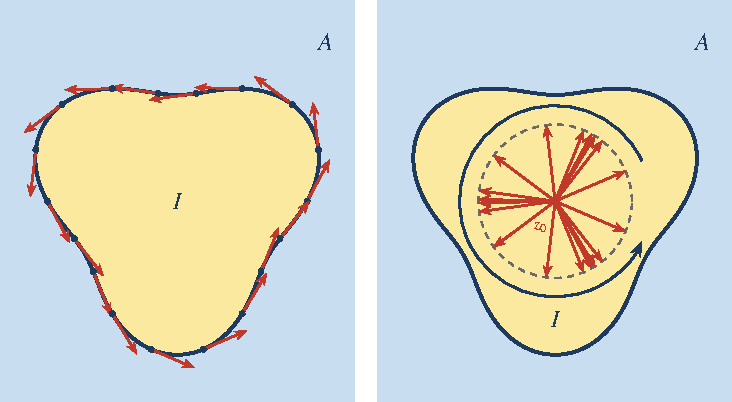
\includegraphics{papers/jordan/images/tangentenwindungszahl.pdf}
    \caption{Drehung der Tangenten beim Umlauf einer Kurve (links). Die Nettodrehung der Tangentenvektoren $\tau(t)$ entlang der Kurve $\gamma$ ist $2\pi$, was der Umlaufzahl $n(\gamma, z_0) = 1$ entspricht (rechts).}
\end{figure}

Es gibt mehrere Beweise für den Hopfschen Umlaufsatz, wobei manche deutlich simpler sind als andere.
Heinz Hopf selbst bewies den Satz in seinem Artikel ``Über die Drehung der Tangenten und Sehnen ebener Kurven''\cite{jordan:Hopf1935}, publiziert in der zweiten Ausgabe des Journals ``Compositio Mathematica'', über ein stetiges Deformationsargument über ein Dreieck im Parameterraum einer Funktion $f$.

Beweise des Hopfschen Umlaufsatzes, welche auf den Satz von Jordan zurückzuführen sind, sind nicht trivial, aber bekannt. 
Ein Beispiel für solch einen Beweis ist in Manfredo do Carmos ``Differential Geometry of Curves and Surfaces'' \cite{jordan:doCarmo1976} zu finden. 
Er beruht auf einer Homotopie zwischen der Sehnen-Richtungs-Abbildung
\[
    \hat{\gamma}(s,t) = \frac{\left( \gamma(t) - \gamma(s) \right)}{\lVert \gamma(t) - \gamma(s) \rVert}
\] 
und der Tangentenabbildung 
\[
    \tau(t) = \frac{\gamma'(t)}{\lVert \gamma(t) - \gamma(s) \rVert}
\] 
. 

Wir verwenden den Hopfschen Umlaufsatz, ohne ihn in diesem Text selbst zu beweisen.

\begin{figure}
    \centering
    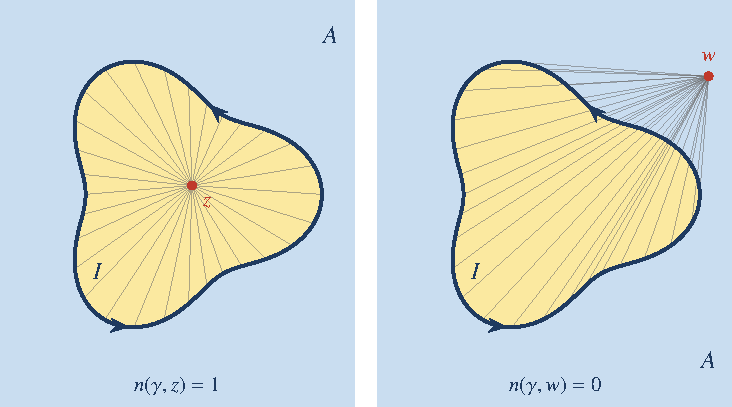
\includegraphics{papers/jordan/images/umlaufzahl.pdf}
    \caption{Konstruktion der Umlaufzahl am Beispiel eines Punkts innerhalb (links) und ausserhalb (rechts) einer Jordan-Kurve.}
\end{figure}

Der Beweis des Satzes von Jordan für reell-analytische Kurven unter Verwendung der Umlaufzahl ist nicht nur deutlich eleganter als der Ansatz basierend auf der Strahlenparität, sondern er zeigt sich auch deutlich robuster und flexibler.
So kann man mit nur geringen Modifikationen den Beweis auf Kurven erweitern, welche moderate Singularitäten besitzen.